


\section{Evaluation}
\label{sec:evaluation}

This section evaluates whether off-the-shelf LLMs can act as useful Roofline triage tools for GPU kernels by predicting runtime \rai from static code features.
We compare two prompting settings used in the paper: \textit{source-only} and \textit{source+SASS}, where the former only provides pre-compilation information to make predictions, while the latter provide post-compilation SASS instructions corresponding to the target kernel of interest for prediction.
We focus on three LLMs in this evaluation, \gptfivefour, \gptoss, and \opus.
Due to the expensive query costs associated with the \gptfivefour and \opus LLMs, we only perform \rai predictions once for each kernel across all four target GPUs.
Given the large number ($254*4=1016$) of GPU-kernel combinations that we sample for each LLM, we are able to get a sufficient understanding of their overall performance.
% Because the \rai-percent-error distributions contain extreme outliers, we emphasize medians, interquartile behavior, and balanced classification accuracy rather than prediction means.
% \textit{Unless otherwise stated, the figures below are all based on predicting the \rai of kernels with a \textbf{non-zero expected \rai value}; this prevents skewing the data towards low \rai errors by kernels that do not perform any FLOP work or DRAM reads/writes.}
% We later perform an analysis including all kernels, regardless of \rai value.
Given the heavy-tailed \rai-percent-error distributions, we emphasize medians, interquartile behavior, and balanced classification accuracy.
\textit{Unless otherwise stated, the figures below only include kernels with non-zero expected \rai values; we later analyze all kernels, including zero-\rai cases.}



\begin{figure}[h]
    \centering
    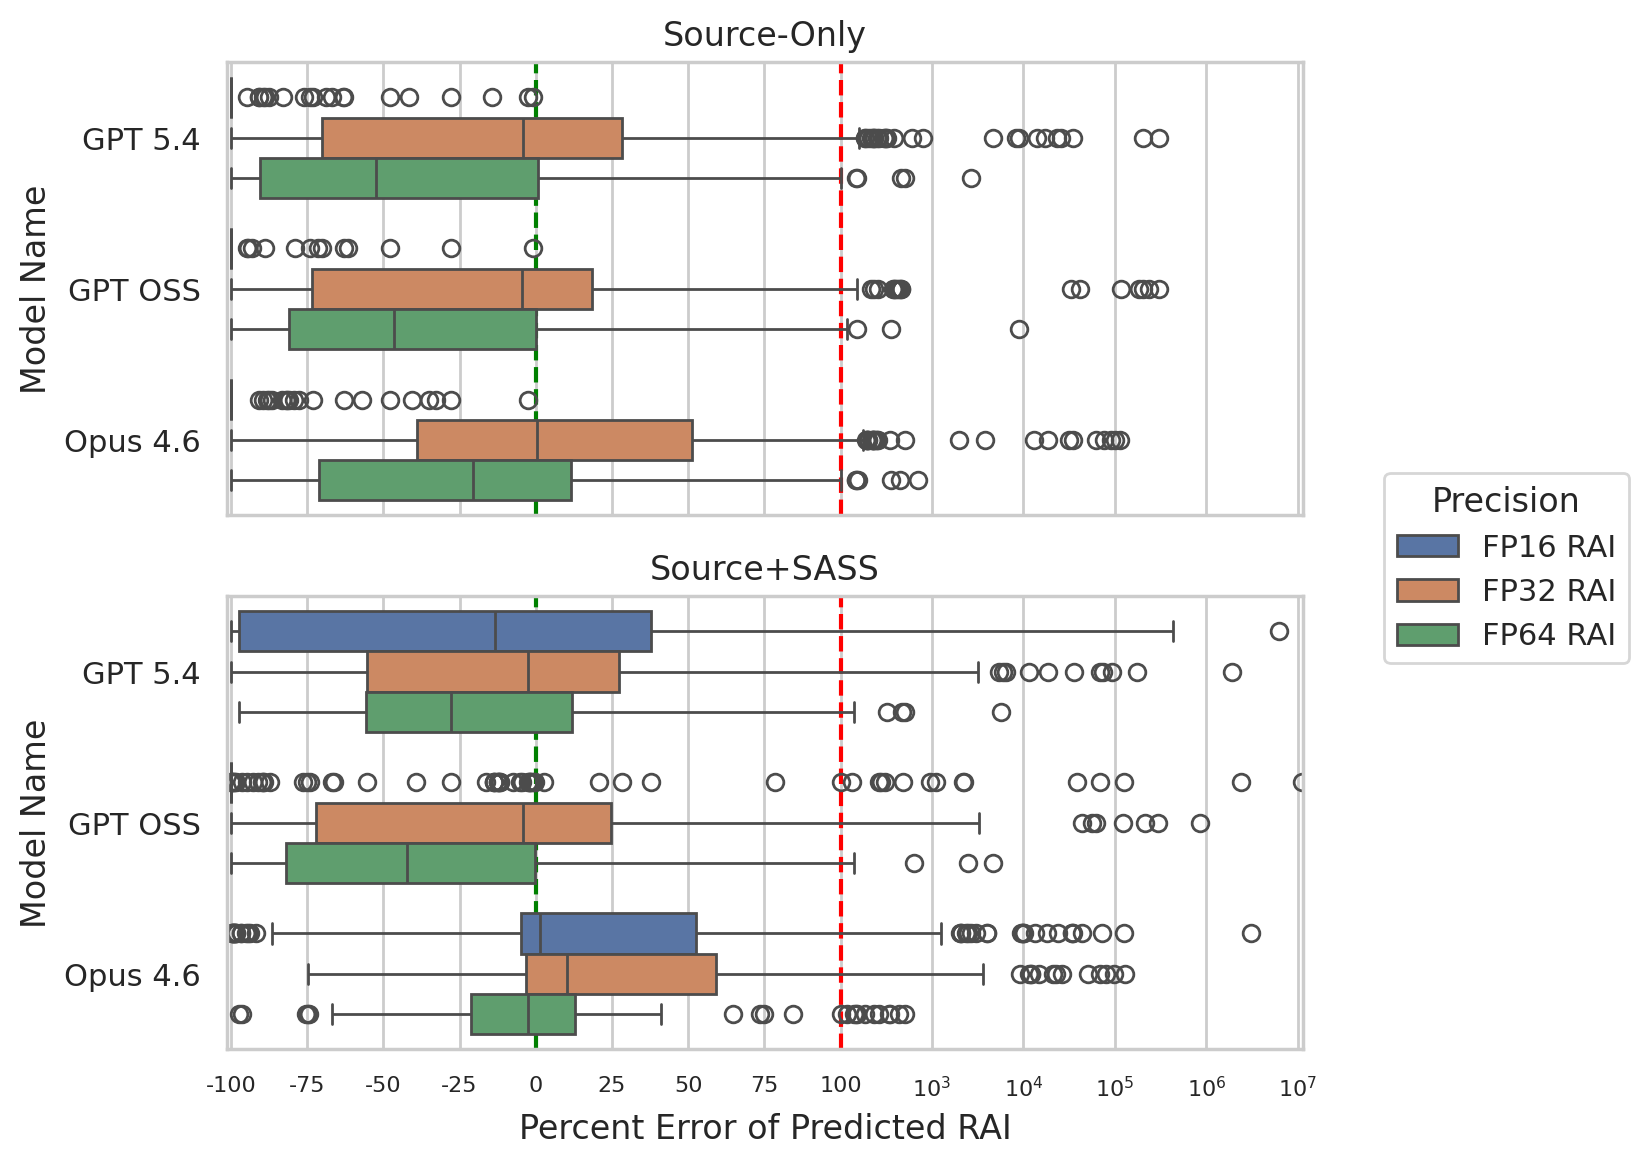
\includegraphics[width=0.95\linewidth]{figures/figure11_ai_percent_difference_boxplots.png}
    \caption{Distribution of \rai percent error for non-zero ground-truth cases, grouped by model and prompt setting across FP16/32/64 predictions.
    The hybrid linear-log x-axis expands the $\pm 100\%$ region while retaining large outliers; values closer to 0 are better.
    Adding post-compilation information helps the stronger models most, especially for FP16.}
    %\caption{Distribution of \rai percent error grouped by prompt type (top/bottom) and model (y-axis) across FP16, FP32, and FP64.
    %A hybrid linear-log scale emphasizes errors within $\pm 100\%$ while still showing larger outliers aggregated across all four GPUs and both runtimes.
    %}
    % \caption{Distribution of \rai percent error grouped by prompt type (top/bottom subplots) and model name (y-axis) across the three FLOP precisions (legend).
    % The plot is on a hybrid linear-log scale to emphasize the percent errors between $\pm 100\%$ in a linear scale, with errors beyond 100\% (the vertical red dashed indicator line) appearing on the log scale.
    % The errors shown for each model are aggregated from the predictions done on all four GPUs for both CUDA and OpenMP codes; this gives us a high-level view of the per-model prediction errors.
    % }
    \label{fig:per_model_ai_percent_diffs}
\end{figure}

\textbf{Per-Model \& Prompt Type Prediction Error.}
\autoref{fig:per_model_ai_percent_diffs} is a box-and-whisker visualization of the \rai percent prediction error for each FLOP precision and prompt type across the three tested LLMs: \gptfivefour, \gptoss, and \opus. 

There are a few trends to note:
\textbf{(1)} The FP16-\rai prediction error significantly improves for \gptfivefour and \opus when the SASS instructions are introduced.
From a median of -100\% on both, to a median of -13.5\% and 1.24\%, respectively.
\textbf{(2)} Unfortunately, the \gptoss model does not appear to make much use of the extra SASS information, given that it's median error stays at -100\% for FP16-\rai predictions, meanwhile it's FP32 and FP64 IQRs stay mostly the same.
\textbf{(3)} The cheap \gptoss and expensive \gptfivefour have very similar prediction distributions when given \sourceonly prompts, suggesting that in cases where a user can not get the SASS instructions for their kernel, the \gptoss model is a cost-effective alternative to querying \gptfivefour.
\textbf{(4)} Overall, the best performing model is \opus when prompted with \sourceSASS due to it's tighter IQRs and lower medians across all three FLOP precisions.

Given that the \gptoss model has a high chance of skewing model-aggregate metrics towards appearing more error-prone, we refer to \autoref{tab:nz_rai_results} to discuss the per-GPU and per-runtime prediction errors.
\autoref{tab:nz_rai_results} shows a heatmap of the proportion of non-zero \rai kernels that were predicted within a \pmten and \pmfifty \rai prediction error, where the \pmten acts as a strict error-bound and \pmfifty a more relaxed error-bound that allow us to better understand how well each LLM predicts \rai for each GPU, runtime, and prompt-type combination.
For \autoref{tab:nz_rai_results} we note that on the 3080 and A10 GPUs, the sampled OpenMP kernels did not perform any FP16 instructions, thus those metrics in the table are omitted.


% \autoref{fig:eval_ai_diff_by_model} is a box-and-whisker visualization of the \rai prediction error for each FLOP precision type across three tested LLMs: \opus, \gptoss, and \gptfivefour.
% The plot is on a log scale to more clearly show the prediction errors (predicted minus expected \rai), with the green vertical dashed line indicating an error of 0, while the red dashed lines indicate an error of +/-1.
% The top subplot shows the prediction errors when prompting only with source, while the bottom subplot prompts with source and SASS information.
% The errors shown for each model are aggregated from the predictions done on all four GPUs.
% 
% There are few major trends of note:
% (1) From the IQRs of each boxplot, roughly 50\% of all \rai predictions are within a +/-1 error away from the ground-truth profiled \rai.
% FP32-\rai (orange boxes) having the lowest overall prediction errors, followed by FP64-\rai (green boxes).
% (2) FP16-\rai (blue boxes) is always under-predicted from the \sourceonly setting, where the introduction of SASS instructions greatly ameliorates mispredictions.
% (3) The cheap \gptoss and expensive \gptfivefour have very similar prediction distributions in the \sourceonly setting, yet \gptoss fails to adequately use the post-compilation information in the \sourceSASS setting to improve the FP16-\rai error, given by it's FP16-\rai IQR still in the negative on the \sourceSASS prompts.

% Although the expensive models perform well in the \rai prediction task for many codes, there still exist many outlier cases with severe over- and under-prediction. 
% In the case of FP64-\rai predictions, given how the balance points listed in \autoref{tab:gpu_specs} range from 0.6 to 10, an \rai misprediction over or under by 1 could be the difference between a correct compute- or bandwidth-bound classification.
% We discuss this further in the next subsection. 

\input{listings/percent_summary_table}


% \begin{figure}[t!]
%     \centering
%     
\includegraphics[width=0.9\linewidth]{figures/figure1_ai_difference_boxplots.png}
%     \caption{Distribution of predicted minus expected Roofline Arithmetic Intensity, grouped by model and split into source-only and source+SASS settings. Separate boxes correspond to FP16, FP32, and FP64, and the dashed line marks zero error.}
%     \label{fig:eval_ai_diff_by_model}
% \end{figure}




% \begin{figure}[h!]
%     \centering
%     
\includegraphics[width=0.9\linewidth]{figures/figure3_ai_difference_boxplots_by_gpu.png}
%     \caption{Distribution of predicted minus expected arithmetic intensity grouped by target GPU and split into source-only and source+SASS settings.}
%     \label{fig:eval_ai_diff_by_gpu}
% \end{figure}

\textbf{Per-Runtime Prediction Error.}
In considering the CUDA/OpenMP runtime prediction errors, \autoref{tab:nz_rai_results} shows a few general trends:
\textbf{(1)} When making \sourceonly predictions with the OpenMP runtime, all the models struggle to make FP16-\rai predictions, given by the zero proportion of kernels that are predicted within the \pmfifty error range.
When it comes to the CUDA runtime under the same \sourceonly FP16-\rai conditions, the LLMs still struggle across all GPUs, but at the very least tease out a couple of close \rai estimates due to the non-zero \pmfifty error ranges.
This aligns with the fact that FP16 instructions often get inserted post-compilation, where prompting with \sourceSASS makes the instructions more apparent.
\textbf{(2)} If a choice needed to be made between using LLMs to predict on a CUDA or an OpenMP runtime, said choice is dependent on LLM model and FLOP precision of the target kernel.
Across GPUs, \opus is better at predicting FP32-based CUDA kernels because an average of 73.6\% of CUDA kernels have at most a \pmfifty error, while an average 66.1\% of OpenMP kernels have at most a \pmfifty error.
We see a similar trend for \gptfivefour, in favoring CUDA for FP32-based kernels.
As for FP64-based kernels, \opus does about the same on either runtime, where \gptfivefour does better for OpenMP codes.
\textbf{(3)} If LLM query budget is a consideration, the \gptoss model exhibits the same trend as its more recent \gptfivefour, where it's better at predicting FP64-based OpenMP codes, and FP32-based CUDA codes.

From these results, the general rule-of-thumb would be that the LLMs will give better predictions on CUDA codes that are FP16/FP32-heavy, and better predictions on OpenMP codes that are more FP64-heavy.


\textbf{Per-GPU Prediction Error.}
From the perspective of per-gpu error, \autoref{tab:nz_rai_results} shows that prediction error is not the same across GPUs, with A100 and H100 predictions being the most accurate when made by the \opus and \gptfivefour models.
For FP32-\rai predictions, the LLMs tend to predict the worst on the A10 GPU across both runtimes and prompt types, evidenced by how at best 15.7\% of the kernels have a \pmten error when predicted by \opus, however this misprediction effect seems to peter out at the \pmfifty error range, with the proportion of A10 kernels more closely matching the other GPUs.
These results align with the fact that that the 3080 and A10 GPUs have smaller 5MB and 6MB L2 cache sizes, respectively, therefore the LLMs have to account for L2 cache misses serviced by GPU DRAM---implying higher DRAM Bytes read---which can easily throw off the denominator of the \rai calculation.
In the A100 and H100 with larger 40MB and 50MB L2 caches, respectively, the LLMs can more correctly assume that total DRAM writes end up being small because the working set of memory is more likely to stay in the L2 cache. 
The takeaway here is that LLMs still struggle to accurately account for caching effects that impact the memory traffic on GPUs with smaller caches, thus leading to worse predictions.
If possible, LLM-based \rai predictions should be done on GPUs with larger caches for less error-prone results.

% For FP64-\rai predictions, the \pmten proportion is lower across the board in comparison to the FP32-\rai, however when we consider the more relaxed \pmfifty error, we see a larger proportion of predictions (often 10-20\% more) 
% \autoref{fig:eval_ai_diff_by_gpu} shows the same \rai error metric as \autoref{fig:eval_ai_diff_by_model}, however it is broken down by GPU model and is an aggregate across all three LLMs.
% We can again notice that about 50\% of the predictions are within a small +/-1 error range for the more straight-forward FP32 and FP64 predictions, however when doing \sourceonly predictions, the FP16 errors (blue boxes) are much larger, where the LLMs are severely undercounting across all architectures.
% This is primarily due to how the compiler inserts more FP16 ops into the A100 and H100 kernels, which only becomes apparent upon inspection of SASS.
% The introduction of SASS improves predictions across the A100 and H100 GPUs, primarily because it makes abundantly clear to the LLMs the quantity of FP16 instructions that get compiled into the program.
% An unexpected result is how the \sourceSASS configuration doesn't improve the FP64 predictions (green boxes) by much across 




% \autoref{fig:eval_ai_diff_by_runtime} shows the same box-and-whisker error data split by CUDA and OpenMP runtime, aggregated over the LLM models and GPU archs.
% There are two major points that should be highlighted:
% \begin{enumerate}
%     \item For either runtime, the prediction errors are quite similar, indicating that current LLMs can handle reasoning about either runtime just as equally.
%     \item The inclusion of SASS lowers the error of FP16-\rai predictions for both runtimes, pushing the IQR into the +/-1 error band.
% \end{enumerate}
% As for the FP64 and FP32 errors, there is not too much of a difference.


% \begin{figure}
%     \centering
%     
\includegraphics[width=0.9\linewidth]{figures/figure4_ai_difference_boxplots_by_runtime.png}
%     \caption{Distribution of predicted minus expected arithmetic intensity grouped by runtime (CUDA versus OpenMP) and split into source-only and source+SASS settings.}
%     \label{fig:eval_ai_diff_by_runtime}
% \end{figure}


\begin{figure}[t!]
    \centering
    %
\includegraphics[width=0.9\linewidth]{figures/figure2_ai_bound_confusion_heatmaps.png}
    %\caption{Confusion heatmaps comparing expected and predicted \rai bound class: Compute-Bound (CB) and Bandwidth-Bound (BB). 
    %Each cell is annotated with FP16, FP32, and FP64 code percentages corresponding to the proportion of kernels that were expected to be a part of a bound-class that were predicted in another bound-class; intuitively, darker main-diagonal cells indicate stronger agreement between expected and predicted Roofline class.}

    
\includegraphics[width=0.95\linewidth]{figures/figure2_5_ai_bound_confusion_heatmaps_with_zero.png}
    \caption{Confusion heatmaps for the three \rai classes used in the paper: zero-valued, compute-bound, and bandwidth-bound.
    Subplot rows correspond to models and columns to prompt settings; each cell reports FP16, FP32, and FP64 percentages for that expected-versus-predicted class pair.
    Darker diagonal cells indicate stronger agreement. 
    Post-compilation information most clearly improves compute-bound and bandwidth-bound classification for the stronger models.}
    %\caption{Confusion heatmaps comparing the expected and predicted \rai classification accuracy: Zero-value, Compute-Bound (\compbound), and Bandwidth-Bound (\bandbound).
    %Each cell is annotated with FP16, FP32, and FP64 code percentages corresponding to the proportion of kernels that were predicted to be a part of a particular classification. 
    %Each subplot row corresponds to a particular LLM, while each subplot column corresponds to prompting \sourceonly or with \sourceSASS.
    %Intuitively, darker main-diagonal cells indicate stronger agreement between expected and predicted \rai classifications.
    %}
    \label{fig:eval_ai_bound_heatmaps}
\end{figure}


%%% Need to change this plot to include the zero cases

\textbf{\rai Classification Accuracy.}
% The previously-discussed results focused on the predictions made for the kernels with non-zero expected \rai values.
% We now shift our focus to study both zero and non-zero expected-value \rai kernels; we do so from the perspective of correct binary Roofline classification accuracy.
We now extend the analysis to both zero and non-zero expected-value \rai kernels by evaluating Roofline classification accuracy.
The benefit of this perspective is that although a large number of \rai predictions may have a large percent error of \pmfifty, if they are on the correct side of each GPU Roofline's balance point, they will be considered correctly classified as either Bandwidth-Bound (\bandbound, less than balance point) or Compute-Bound (\compbound, greater than balance point).
Having a correct classification can dramatically change the types of optimizations applied to a kernel during tuning; if \compbound, the optimizer may focus on doing more FLOP work for each byte of memory moved, and if \bandbound, coalescing memory movement for each FLOP performed).
There exists a third \rai classification: we consider a \rai value of \textit{zero} its own class so as not to skew the \bandbound accuracy results.
% Given that a \rai prediction error falls within the +/-1 range for about 50\% of the tested codes, we consider how this affects the \rai classification of a kernel as being Bandwidth-Bound (\bandbound) or Compute-Bound (\compbound).
\autoref{fig:eval_ai_bound_heatmaps} depicts the classification accuracy of the predicted \rai results, where the confusion tables show the percent of cases that were predicted as zero-valued, \bandbound, or \compbound across all three models (rows) when they were prompted with \sourceonly or with \sourceSASS (columns). 
From the figure we can note a few points:
\textbf{(1)} Prompting on all three models with \sourceonly inputs, causes many \bandbound and \compbound kernels to be misclassified as having 0 FP16-\rai. 
This effect is consistent with the previous results in \autoref{tab:nz_rai_results} and \autoref{fig:per_model_ai_percent_diffs}.
The prediction accuracies in all the cells are very similar between LLMs with \sourceonly prompting, implying that if a user does not have SASS instructions to add to their prompt, they can get similar \rai classification results from both the economical and premium LLMs.
\textbf{(2)} Another repeat trend is how prompting with \sourceSASS significantly improves correct prediction accuracy across LLMs, with \opus seeing the best improvements in accuracy of 95\% or greater for the \compbound and \bandbound kernels.
% \textbf{(3)} Across all models and prompt types, the Zero-class classification is frequently correct, scoring consistently-high accuracies.
% Unfortunately, when we prompt with \sourceSASS, all the models begin to incorrectly classify 5-15\% more of the Zero-class FP32 kernels as \bandbound.
% We found this effect was due to X.

The takeaway here is that across all three LLMs, \textbf{(a)} with simple \sourceonly prompting, a fiscally-conscious user may stick to \gptoss for \rai classifications, and \textbf{(b)} the inclusion of SASS instructions improves classification accuracy for the expensive LLMs, especially on \compbound kernels.
% This is a common trend of ``\textit{you-get-what-you-paid-for}'', where the classification accuracy directly improves from cheapest to most expensive LLM.

%Across all models, the inclusion of SASS improves the FP16 CB prediction accuracy significantly.
%In the cases of \opus and \gptfivefour, they go from 100\% misprediction to 100\% and 76\% correct predictions respectively.
%Unfortunately, in the case of \gptoss, the improvements are meager, and can even cause a drop in accuracy as seen for the FP64 case. 





\textbf{Error-Prone Code Features.}
\autoref{fig:codeFeatureAssociationHeatmap} shows a \rai prediction error attribution heatmap split by prompt-type and LLM model, using the Cliff's Delta metric defined at the end of \autoref{sec:methodology}.
For this error analysis, we purposely include the kernels that were predicted on with expected \rai values of zero, as the Cliff's Delta metric is robust to skewness.
For reference, the different categories of code feature flags are described in more detail in Appendix \autoref{sec:codeFeatureCategoriesAppendix}.

What we end up finding is that across both runtimes, prompt types, and GPU types, the largest chances of \rai mispredictions occur when FLOP division, FLOP subexpressions, special FLOP math functions, and loop-invariant FLOPs are present.
FLOP division introduces not only new FLOPs into the SASS, but also data-dependent branching to implement the Newton-Raphson root-finding approach used in the IEEE FLOP division spec \cite{IEEEStandardFloatingPoint2019}. 
Similarly, \textit{special} (i.e.: transcendental) math functions like \texttt{sin} and \texttt{cos} also introduce new FLOPs into the SASS that the LLMs much account for.
On the other hand, \textit{common FLOP subexpression elimination} and \textit{loop-invariant FLOP hoisting} remove repeat operations from the SASS, easily allowing an LLM to overcount repeat work during static analysis.
Given the very direct influence these features have on the final number of floating point operations that get included into a kernel's instructions, it makes sense that they can lead to the highest misprediction errors.

On the other end of the spectrum, the features of \textit{deterministic grid/block size} detect whether the grid and block size can be statically determined via constant propagation of literals, macros, and command-line arguments supplied during prompting.
\autoref{fig:codeFeatureAssociationHeatmap} show that across all cases, these two features tend to lean towards the negative Cliff Delta values, yet hang around 0, indicating that there are only slightly more cases where the presence of these features has a lower \rai error than without.

The takeaway from this analysis is that \textbf{(a)} regardless of LLM and prompt-type, the same code features contribute to the most (and least) \rai prediction errors, and \textbf{(b)} users should try to minimize the occurrence of FLOP divison, subexpressions, special math functions, and loop-invariant ops to maximize the chances of correct LLM-based \rai predictions; similarly, maximizing the ease with which an LLM could determine grid/block size can aid in accurate predictions.

% This intuitively makes sense, as being able to correctly determine the grid and block sizes leads to proper thread count prediction, allowing for accurate FLOP and DRAM read/write count predictions.

% \autoref{fig:promptFeatureAssociationHeatmap} and \autoref{fig:gpuFeatureAssociationHeatmap} show a \rai prediction error attribution heatmap split by prompt type and GPU, respectively, for each runtime, using the Cliff's Delta metric defined at the end of \autoref{sec:methodology}. 
% For this error analysis, we purposely include the kernels that were predicted on with expected \rai values of 0, as the Cliff's Delta metric is robust to skewness.
% For reference, the different categories of code feature flags are described in more detail in Appendix \autoref{sec:codeFeatureCategoriesAppendix}.
% 
% What we end up finding is that across both runtimes, prompt types, and GPU types, the largest chances of \rai misprediction occur when FLOP division, FLOP subexpressions, special FLOP math functions, and loop-invariant FLOPs are present.
% FLOP division introduces not only new FLOPs into the SASS, but also data-dependent branching to implement the Newton-Raphson root-finding approach used in the IEEE FLOP division spec \cite{IEEEStandardFloatingPoint2019}. 
% Similarly, \textit{special} (i.e.: transcendental) math functions like \texttt{sin} and \texttt{cos} also introduce new FLOPs into the SASS that the LLMs much account for.
% On the other hand, \textit{common FLOP subexpression elimination} and \textit{loop-invariant FLOP hoisting} remove repeat operations from the SASS, easily allowing an LLM to overcount repeat work during static analysis.
% Given the very direct influence these features have on the final number of floating point operations that get included into a kernel's instructions, it makes sense they can lead to the highest misprediction errors.
% 
% One of the most salient distinctions that can be made from these plots is how the presence of \textit{calls to helper functions} (i.e.: calling a \texttt{\_\_device\_\_} function in CUDA, or a plain function call in an OpenMP parallel region), introduces much less errors for CUDA codes than for OpenMP.
% It turns out that this is caused by TODO.
% This outcome aligns with how \cite{timeMattisonPaperwithOpenMPStudy} found that OpenMP is less present in LLM training data (re-write this sentence).

% Lastly, the features of \textit{deterministic grid/block size} detect whether the grid and block size can be statically determined via constant propagation of literals, macros, and command-line arguments supplied during prompting.
% \autoref{fig:promptFeatureAssociationHeatmap} and \autoref{fig:gpuFeatureAssociationHeatmap} show that across all cases, these two features tend to lean towards the negative Cliff Delta values, yet hang around 0, indicating that there there are only slightly more cases where the presence of these features has a lower \rai error than without.
% This intuitively makes sense, as being able to correctly determine the grid and block sizes leads to proper thread count prediction, allowing for accurate FLOP and DRAM read/write count predictions.

\begin{figure}
    \centering
    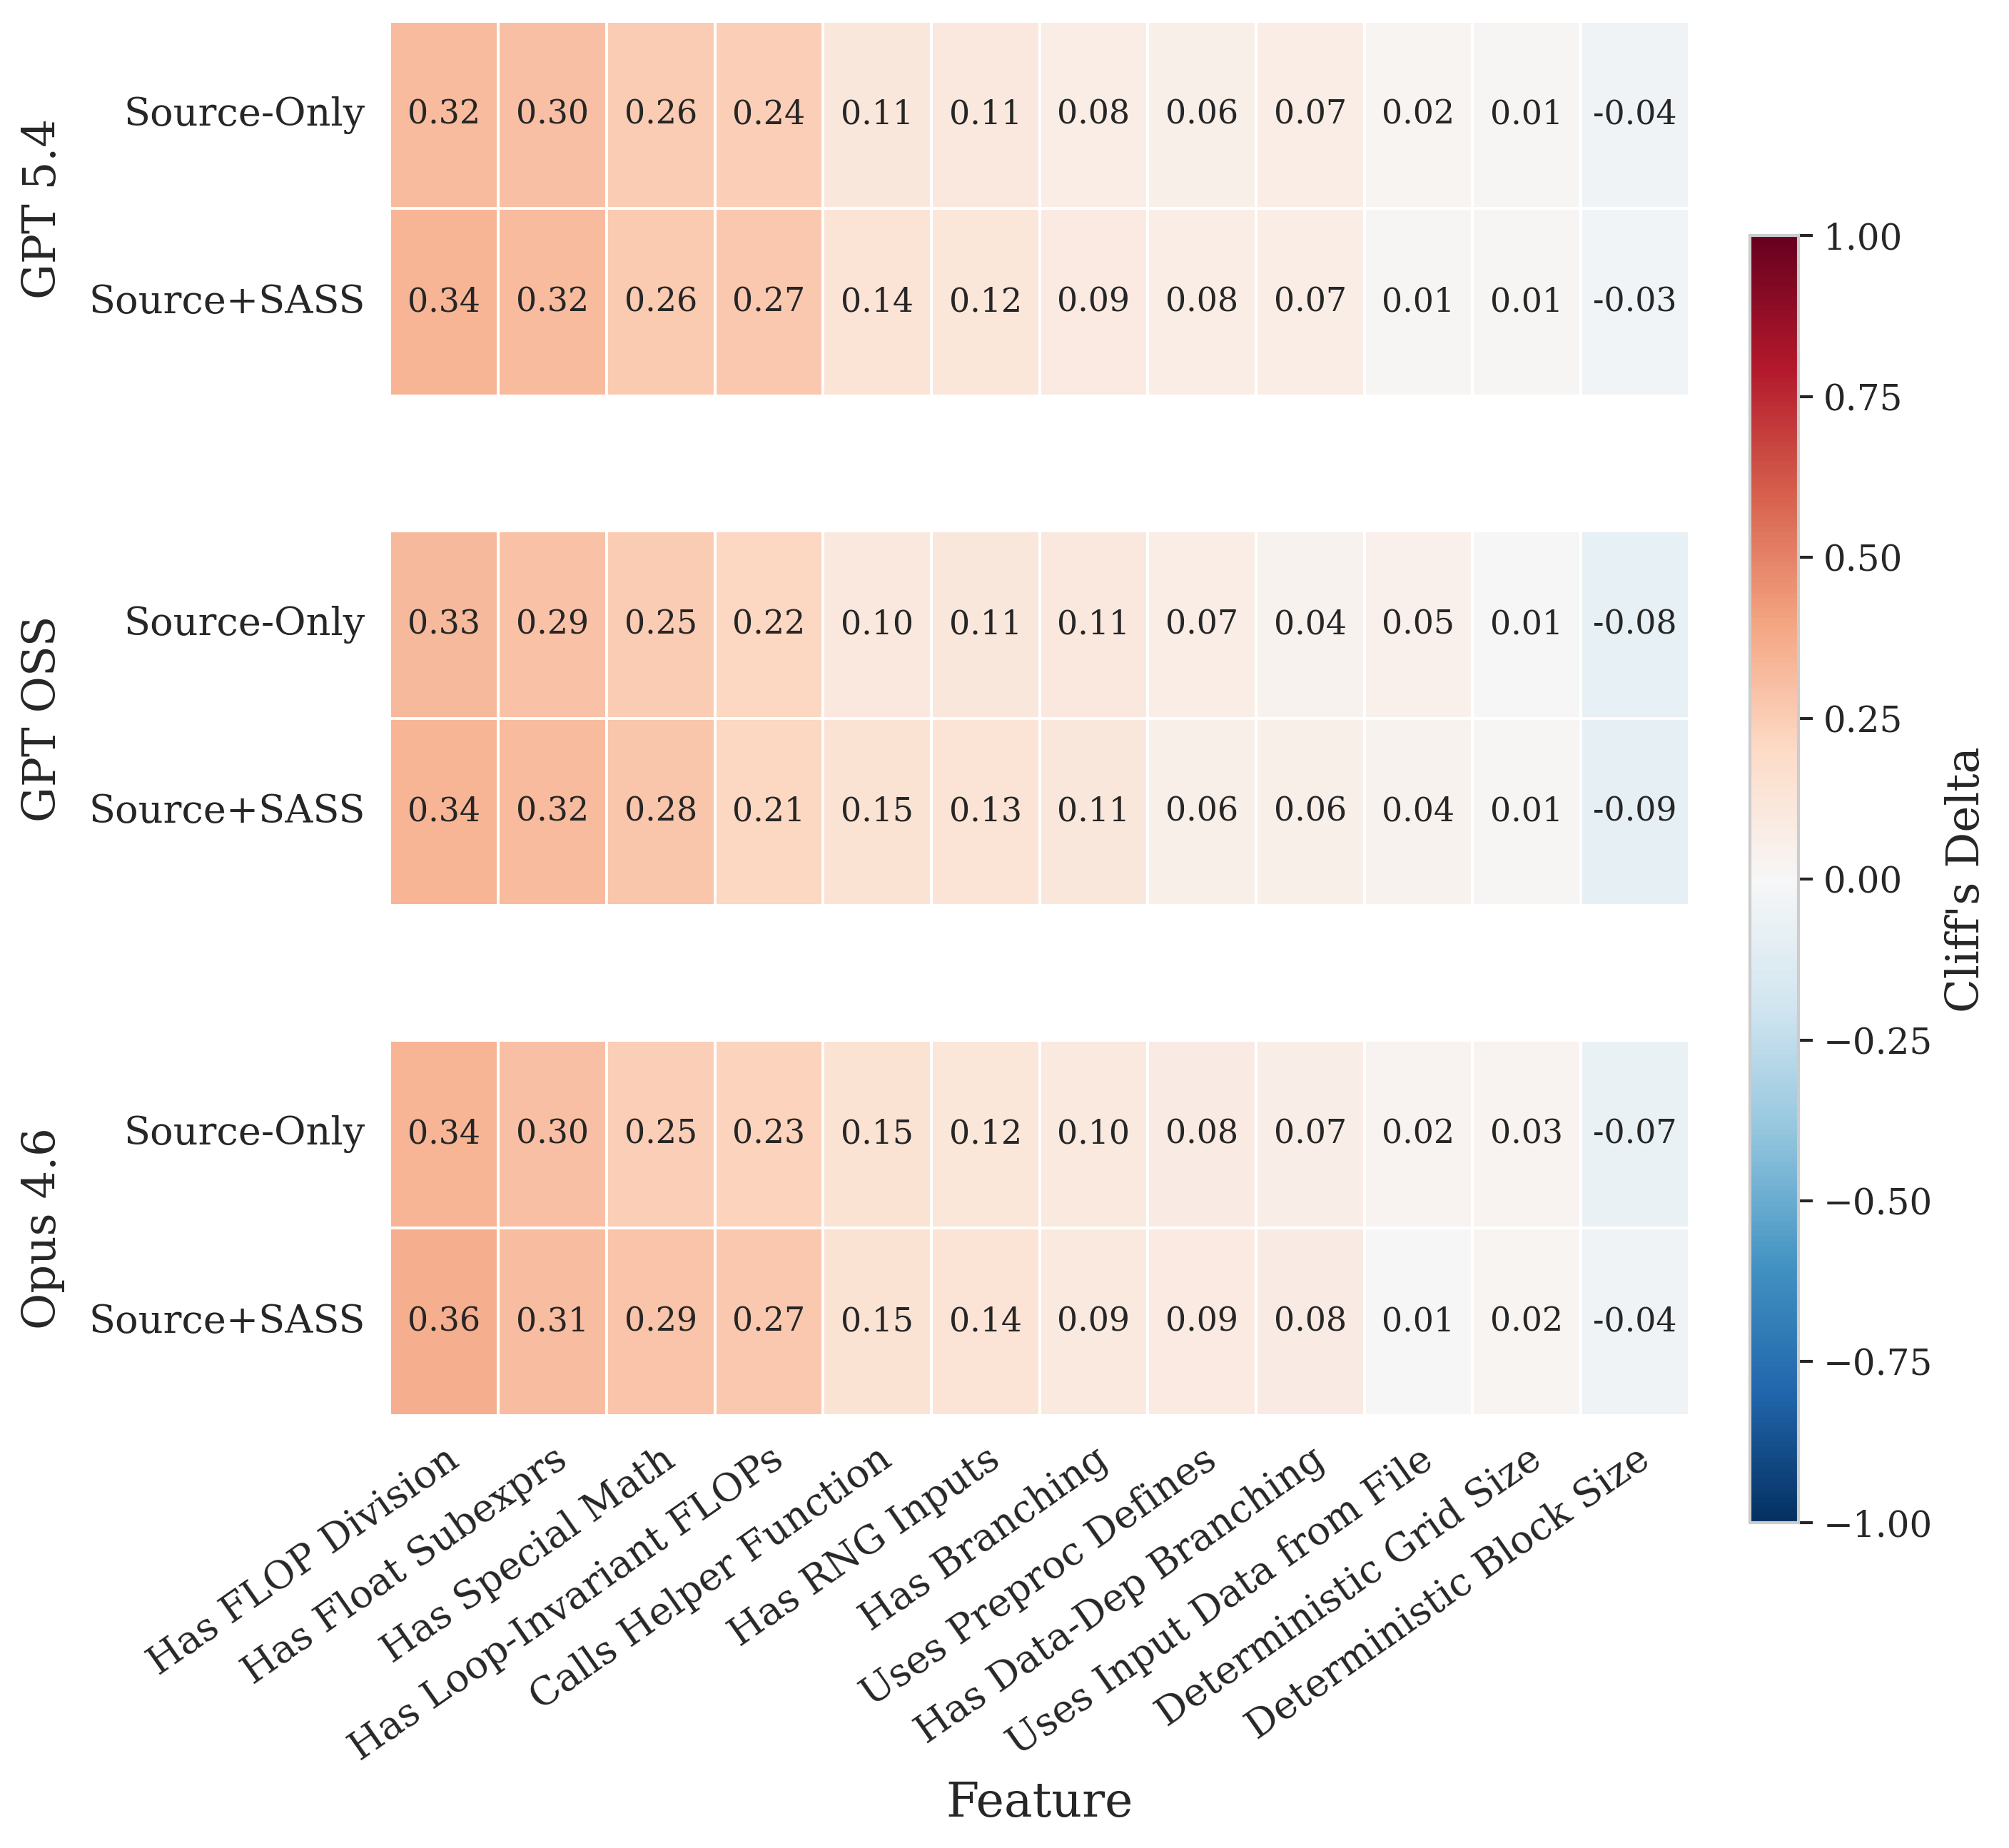
\includegraphics[width=0.95\linewidth]{figures/figure1_model_feature_association_heatmap.png}
    \caption{Cliff's Delta heatmap relating source features to absolute \rai error, split by prompt type and model. 
    Positive values mean the feature is associated with larger errors, negative values with smaller errors.
    FLOP division, reusable subexpressions, special math functions, and loop-invariant work are the most consistent error drivers.}
     %\caption{Code feature error attribution heatmap split by prompt type and model name.
     %Errors are consistent across models and prompt types, with the presence of \textit{FLOP division} and \textit{float subexpressions} leading to a higher chance of \rai mispredictions.}
    \label{fig:codeFeatureAssociationHeatmap}
\end{figure}

% \begin{figure}
%     \centering
%     
\includegraphics[width=0.95\linewidth]{figures/runtime_feature_association_heatmap.png}
%     \caption{Code feature error attribution heatmap split by prompt type and runtime.
%     Errors are similar across both prompting types, with the presence of \textit{FLOP division} and \textit{float subexpressions} leading to a higher chance of \rai mispredictions.}
%     \label{fig:promptFeatureAssociationHeatmap}
% \end{figure}
% 
% \begin{figure}
%     \centering
%     
\includegraphics[width=0.95\linewidth]{figures/gpu_feature_association_heatmap.png}
%     \caption{Code feature error attribution heatmap split by GPU and runtime.
%     Errors are similar across all prompting types, with the presence of \textit{FLOP division} and \textit{float subexpressions} leading to a higher chance of \rai mispredictions.}
%     \label{fig:gpuFeatureAssociationHeatmap}
% \end{figure}








\textbf{LLM Cost and Time Analysis.}
\autoref{fig:costDistrib} shows query cost distributions (in USD) by model and prompt type.
We focus on distinguishing the costs between prompt types, as including SASS instructions increases the amount of tokens each LLM has to process, thus directly increasing cost.
\gptoss is by far the cheapest, with a median cost of \$0.001 per query and under \$3 for roughly 2000 queries.
\gptfivefour is next at \$0.020/\$0.031 median cost for \sourceonly/\sourceSASS, while \opus is highest at \$0.068/\$0.107 and about \$160 total.
This cost ranking closely matches predictive performance: \opus and \gptfivefour are more accurate, but far more expensive.
% \autoref{fig:costDistrib} shows the distribution of query costs (in USD) for each of the prompt types across the three sampled LLMs.
% The right-side margin shows the summed cost across all samples.
% The input/output query token costs are described in \autoref{tab:llm_comparison}, and set by the LLM providers.
% What we can notice is that the \gptoss model is incredibly cost-effective, with a median cost-per-query of \$0.001 for both \sourceonly and \sourceSASS prompting; only costing less than \$3 to make about 2000 queries.
% The next cheapest model is \gptfivefour, with a median cost of \$0.020 and \$0.031 for \sourceonly and \sourceSASS prompts, respectively; costing cumulatively \$47 to perform all the queries. 
% The most expensive is the \opus model, with median costs of \$0.068 and \$0.107 for \sourceonly and \sourceSASS, respectively; costing cumulatively \$160 for the same queries as the other models.
% This cost inequality aligns closely with the predictive performance of the models, where the most expensive (\opus and \gptfivefour) LLMs make better predictions than the cheaper/inaccurate \gptoss.

\begin{figure}[t!]
    \centering
    
\includegraphics[width=0.95\linewidth,trim=0 0 0 0.9cm,clip]{figures/plot3_cost_distribution.png}
    \caption{Per-query cost distribution by model and prompt setting.
    Totals across all queries are shown on the right; adding SASS usually increases cost, while the cheapest model remains orders of magnitude less expensive than the strongest models.}
    %\caption{Query cost distribution across LLMs and prompting type. 
    %Total cumulative costs are shown on the right margin.
    %The queries using \sourceSASS are often more expensive than those of \sourceonly.
    %The \gptoss model is extremely cost-effective in comparison to \gptfivefour and \opus.
    %}
    \label{fig:costDistrib}
\end{figure}

\autoref{fig:timeDistrib} shows the distribution of the query times (in seconds) for each of the prompt types across the three sampled LLMs.
This plot captures the LLM query response generation times, excluding HTTP request travel time.
Surprisingly, \gptfivefour has the lowest inference times, with a median around 10.9 and 12.0 seconds for \sourceonly and \sourceSASS prompting, respectively.
We note that the \gptoss model has the longest query times, with medians around 32.7 and 32.0 seconds for both prompt types, whereas \opus had median times around 21.9 and 29.3 seconds for \sourceonly and \sourceSASS, respectively.
We urge users to jointly consider the monetary, query time, and prediction accuracies of these models when deciding which to use.
Although the \gptoss model is inexpensive, it is not as fast or accurate in comparison to its more recent \gptfivefour counterpart which takes about a third of the time to query, but at about 20x the cost.

\begin{figure}[t!]
    \centering
    
\includegraphics[width=0.95\linewidth,trim=0 0 0 0.9cm,clip]{figures/plot2_query_time_distribution.png}
    \caption{Per-query response-time distribution by model and prompt setting, excluding HTTP latency.
    Adding SASS modestly increases latency for the stronger models, while \gptfivefour is the fastest overall, and \gptoss the slowest.}
    %\caption{Query time distribution across LLMs and prompting type.
    %Querying with or without SASS has little effect on the \gptoss model, however including SASS can cause a median query time increase of about 10\% and 30\% on \gptfivefour and \opus, respectively.}
    \label{fig:timeDistrib}
\end{figure}



%\subsection{RQ1: Generalization Across Architectures}
%
%RQ1 asks whether LLMs can predict arithmetic intensity accurately enough across multiple GPU architectures to remain useful as hardware-free triage tools.
%We answer this question from two perspectives introduced in \autoref{sec:methodology}: (1) quantitative AI error, measured as \textit{predicted AI} minus \textit{expected AI}, and (2) binary Roofline-class agreement, measured by whether the predicted and expected AI values place a kernel on the same side of the architecture-specific balance point.
%
%\autoref{fig:eval_ai_diff_by_model} summarizes the signed AI-error distributions for the two evaluated models under the source-only and source+SASS settings.
%Across both models, the \textbf{median signed FP32 AI error is already close to zero} in the source-only setting, but the tails are heavy, so median absolute AI error is the more stable summary.
%As shown in \autoref{tab:eval_model_summary}, Claude Opus 4.6 is consistently better than GPT-5.4 on quantitative AI prediction: under source-only prompting, its median absolute AI error is 0.321 for FP32 and 0.416 for FP64, compared to 0.746 and 0.590 for GPT-5.4.
%The same ranking holds in the source+SASS setting, where Claude has lower FP32 and FP64 median absolute AI error.
%
%\autoref{fig:eval_ai_bound_heatmaps} shows that \textbf{bound-class agreement is often stronger than raw AI accuracy would suggest}, especially for FP32.
%For source-only prompting, balanced accuracy on FP32 is already high for both models: 0.928 for Claude and 0.889 for GPT-5.4.
%FP64 is noticeably harder, dropping to 0.784 for Claude and 0.679 for GPT-5.4 under source-only prompting.
%FP16 is the clearest failure case for source-only prompting: both models achieve a balanced accuracy of 0.5 because they effectively predict the bandwidth-bound class only, even though raw accuracy remains high due to class imbalance.
%
%\autoref{fig:eval_ai_diff_by_gpu} further shows that generalization is not uniform across architectures.
%For FP32, source-only median absolute AI error ranges from 0.321 on A100 to 0.587 on the RTX 3080, suggesting reasonably stable behavior across GPUs despite large outliers.
%FP64 is more architecture-sensitive: source-only balanced accuracy is 0.788 on the RTX 3080, 0.677 on the A10, but falls to 0.5 on both A100 and H100, indicating that the models frequently miss the compute-bound cases on those architectures.
%Overall, these results suggest that off-the-shelf models are already useful for \textbf{FP32-oriented triage across architectures}, but their FP64 behavior is less reliable and remains strongly architecture-dependent.

% \begin{table*}[t]
%     \centering
%     \caption{Per-model summary of arithmetic-intensity error and bound-class agreement. We report median absolute \rai error because the signed \rai-error distributions are heavy-tailed.}
%     \label{tab:eval_model_summary}
%     \scriptsize
%     \setlength{\tabcolsep}{4pt}
%     \renewcommand{\arraystretch}{1.05}
%     \resizebox{\textwidth}{!}{%
%     \begin{tabular}{llcccccc}
%     \toprule
%     \textbf{Model} & \textbf{Setting} & \textbf{FP16 Med. $|\Delta \mathrm{AI}|$} & \textbf{FP32 Med. $|\Delta \mathrm{AI}|$} & \textbf{FP64 Med. $|\Delta \mathrm{AI}|$} & \textbf{FP16 Bal. Acc.} & \textbf{FP32 Bal. Acc.} & \textbf{FP64 Bal. Acc.} \\
%     \midrule
%     Claude Opus 4.6 & source-only  & 0.507 & 0.321 & 0.416 & 0.500 & 0.928 & 0.784 \\
%     Claude Opus 4.6 & source+SASS  & 0.056 & 0.305 & 0.204 & 0.975 & 0.958 & 0.779 \\
%     GPT-5.4         & source-only  & 0.512 & 0.746 & 0.590 & 0.500 & 0.889 & 0.679 \\
%     GPT-5.4         & source+SASS  & 0.341 & 0.640 & 0.534 & 0.849 & 0.890 & 0.726 \\
%     \bottomrule
%     \end{tabular}%
%     }
% \end{table*}





% \begin{table*}[t]
%     \centering
%     \caption{Architecture-level summary aggregated across both models. FP16 is omitted because the RTX 3080 and A10 contain very few nonzero-AI FP16 samples, making architecture-level comparisons less stable.}
%     \label{tab:eval_gpu_summary}
%     \scriptsize
%     \setlength{\tabcolsep}{4pt}
%     \renewcommand{\arraystretch}{1.05}
%     \resizebox{\textwidth}{!}{%
%     \begin{tabular}{lcccccccc}
%     \toprule
%     \textbf{GPU} & \textbf{FP32 Med. $|\Delta \mathrm{AI}|$} & \textbf{FP32 Med. $|\Delta \mathrm{AI}|$} & \textbf{FP64 Med. $|\Delta \mathrm{AI}|$} & \textbf{FP64 Med. $|\Delta \mathrm{AI}|$} & \textbf{FP32 Bal. Acc.} & \textbf{FP32 Bal. Acc.} & \textbf{FP64 Bal. Acc.} & \textbf{FP64 Bal. Acc.} \\
%      & \textbf{source-only} & \textbf{source+SASS} & \textbf{source-only} & \textbf{source+SASS} & \textbf{source-only} & \textbf{source+SASS} & \textbf{source-only} & \textbf{source+SASS} \\
%     \midrule
%     RTX 3080 & 0.587 & 0.381 & 0.460 & 0.377 & 0.941 & 0.913 & 0.788 & 0.775 \\
%     A10      & 0.522 & 0.521 & 0.420 & 0.225 & 0.843 & 0.883 & 0.677 & 0.703 \\
%     A100     & 0.321 & 0.415 & 0.591 & 0.288 & 0.908 & 0.948 & 0.500 & 0.534 \\
%     H100     & 0.363 & 0.359 & 0.430 & 0.408 & 0.941 & 0.944 & 0.500 & 0.500 \\
%     \bottomrule
%     \end{tabular}%
%     }
% \end{table*}


%\subsection{RQ2: Error Analysis}

%TODO


% \subsection{RQ3: Do Post-Compilation Artifacts Help?}
% 
% RQ3 asks whether providing post-compilation SASS artifacts improves arithmetic-intensity prediction relative to source-only prompting.
% This question is answered by comparing the source-only and source+SASS panels in Figures \ref{fig:eval_ai_diff_by_model}, \ref{fig:eval_ai_bound_heatmaps}, and \ref{fig:eval_ai_diff_by_gpu}.
% The answer is \textbf{yes, but unevenly across precisions and architectures}.
% The strongest gains appear in FP16 and in parts of FP64.
% For Claude, source+SASS reduces the median absolute FP16 AI error from 0.507 to 0.056 and raises FP16 balanced accuracy from 0.5 to 0.975.
% For GPT-5.4, FP16 also improves substantially, though less dramatically, reducing median absolute AI error from 0.512 to 0.341 and increasing balanced accuracy from 0.5 to 0.849.
% 
% FP32 sees more modest gains.
% Claude's median absolute FP32 AI error improves slightly from 0.321 to 0.305, while GPT-5.4 improves from 0.746 to 0.640.
% The corresponding FP32 balanced-accuracy gains are small: 0.928 to 0.958 for Claude and 0.889 to 0.890 for GPT-5.4.
% This suggests that source-level reasoning is already sufficient for many FP32 bound-class decisions, and that SASS mainly helps reduce a subset of remaining quantitative errors.
% 
% FP64 benefits are mixed but still important.
% Claude's median absolute FP64 AI error improves substantially from 0.416 to 0.204, while GPT-5.4 improves more modestly from 0.590 to 0.534.
% On the classification side, Claude's FP64 balanced accuracy remains roughly unchanged (0.784 to 0.779), whereas GPT-5.4 improves from 0.679 to 0.726.
% Thus, SASS is most valuable when source-only prompting misses low-level helper work or compiler-lowered behavior, but it does not uniformly fix every FP64 error mode.
% 
% The architecture-level summary in \autoref{tab:eval_gpu_summary} shows the same pattern.
% For FP64, source+SASS materially lowers median absolute AI error on the A10 (0.420 to 0.225) and A100 (0.591 to 0.288), and it improves FP64 balanced accuracy on the A10 from 0.677 to 0.703.
% For FP32, however, the effect is smaller and sometimes mixed: source+SASS improves the RTX 3080 and H100 slightly, is nearly unchanged on the A10, and increases the median absolute FP32 AI error on A100 from 0.321 to 0.415 even as balanced accuracy improves from 0.908 to 0.948.
% This indicates that post-compilation artifacts are most valuable for recovering \textit{qualitative execution behavior} that affects classification, but they do not always reduce the typical magnitude of quantitative AI error on every device.
% 
% 
% \subsection{Supporting Analysis: CUDA vs. OpenMP}
% 
% As a supporting analysis for RQ1, \autoref{fig:eval_ai_diff_by_runtime} stratifies signed AI error by runtime, separating CUDA kernels from OpenMP target-offload kernels.
% This view helps determine whether the models behave differently when reasoning about native CUDA launches versus compiler- and runtime-mediated OpenMP offload kernels.
% The runtime split reveals a more nuanced pattern than the model-level aggregates.
% For FP32, CUDA has lower median absolute AI error than OpenMP in both settings: 0.345 versus 0.630 under source-only prompting, and 0.337 versus 0.699 under source+SASS.
% However, OpenMP attains slightly higher FP32 balanced accuracy in both settings, indicating that its AI errors are often larger in magnitude but still preserve the correct side of the balance point.
% 
% For FP64, the trend reverses for quantitative error: OpenMP has lower median absolute AI error than CUDA in both settings (0.344 versus 0.814 for source-only, and 0.231 versus 0.413 for source+SASS).
% Yet source+SASS improves FP64 balanced accuracy for CUDA from 0.714 to 0.787, while OpenMP declines slightly from 0.761 to 0.711.
% Taken together, these results suggest that CUDA kernels are typically easier to classify correctly once SASS is available, whereas OpenMP kernels can still have smaller typical AI error even when their bound-class behavior is less stable.
% 
% This subsection does not introduce a new research question; it instead provides additional context for interpreting the model- and architecture-level trends.

